\section{Results}
\label{sec:fld_results}

With the solver introduced in the previous section it can now be run for comparison on the problems, which were used for the $P_N$-method in chapter~\ref{sec:pnmethod} and the diffusion approximation in chapter~\ref{sec:diffusion_approximation}.

The rendering integration aspects to be considered are identical to the diffusion approximation (section~\ref{sec:diffusion_approximation}). As with the diffusion approximation, flux-limited diffusion will give a solution for the zero moment $\phi$ from which the second moment can be recovered using equation~\ref{eq:diffusion_ficks_law}. Both moments can be used to reconstruct the truncated spherical harmonics expansion of the radiance field by using equation~\ref{eq:moment_expansion_L}. The difference to the diffusion approximation solution is that the fluence should be more accurate as the flux-limit constraint had been accounted for.

\subsection{Point Source Problem}
\label{sec:fld_results_pointsource}

At first we consider the point source problem in order to validate the results from the flux-limited diffusion solver and assess its accuracy by comparing against an analytical ground truth solution.
\begin{figure}[h]
\centering
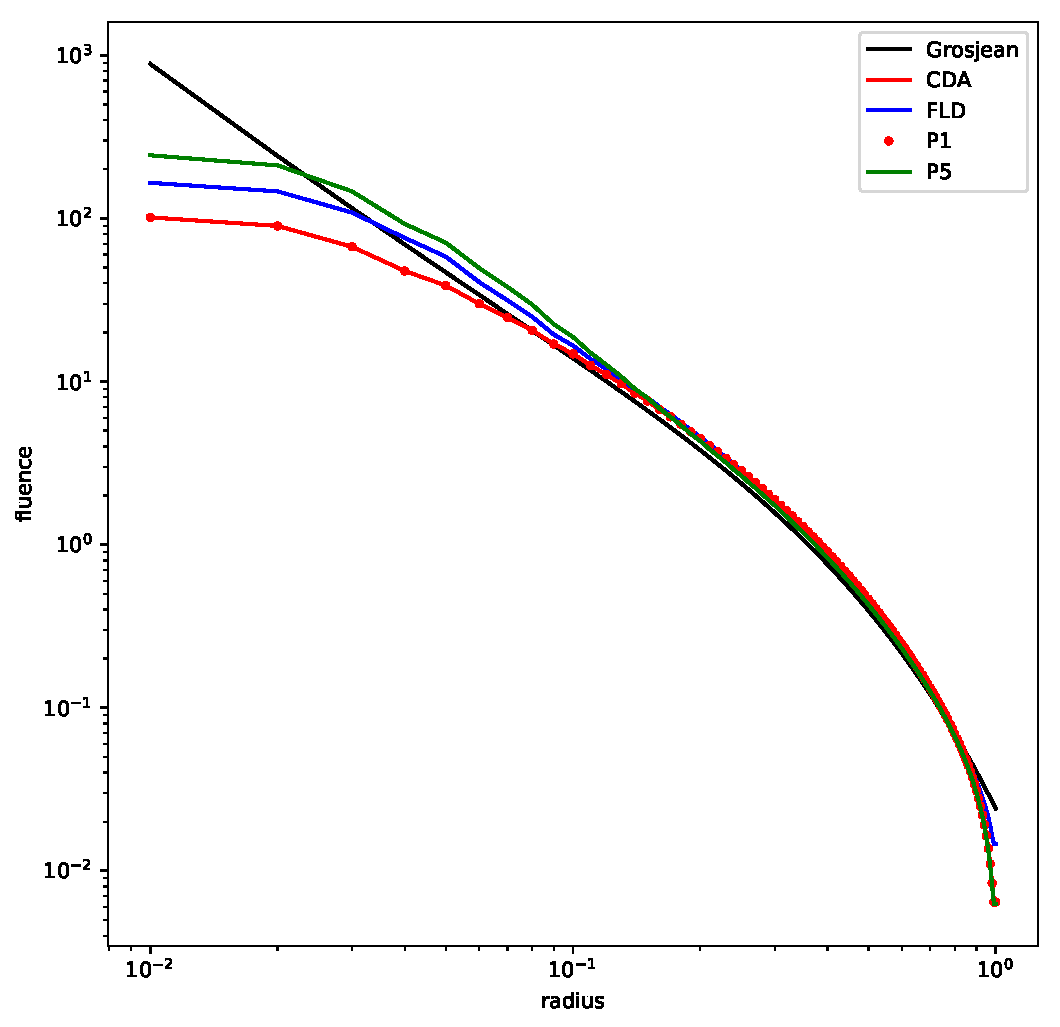
\includegraphics[width=0.7\textwidth]{06_fld/results/fld_result_plot_pointsource.pdf}
\caption{Comparing the solution from flux-limited diffusion (blue) against classical diffusion approximation (red), $P_5$-solution (green) and groundtruth (black). Flux-limited diffusion much closer to the groundtruth and $P_5$-result at much lower computational cost.}
\label{fig:fld_results_pointsource_1}
\end{figure}
As seen in figure~\ref{fig:fld_results_pointsource_1}, the result from flux-limited diffusion agree well with the ground truth and diffusion approximation results. Like with the diffusion approximation, a perfect match to the ground truth is not to be expected as flux-limited diffusion is still an approximation based on the spherical harmonics expansion of the radiative transfer equation truncated after the first moment. However, very close to the point source, the flux-limited diffusion is more accurate than classical diffusion. This is explained by the fact, that the fluence gradient becomes arbitrarily large as the point light is approached, due to the geometry term. This causes the transport measure $R$ to likewise become arbitrarily large, which shows that a pure streaming transport will dominate when coming close to the point source.
% figure of R: (figure~\ref{fig:fld_results_pointsource_2})

In comparison to the results from $P_N$-method and $P_5$ in particular, the $P_N$-method with higher truncation order is more accurate than flux-limited diffusion. This an important observation since it means that increasing the truncation order will alleviate the problems caused by not accounting for the flux-limit constraint. However, flux-limited diffusion has a significcant advantage over $P_N$ due to its computational and memory efficiency.

\begin{table}[!h]
	\centering
	\caption{Performance characteristics of flux-limited diffusion and $P_1$ for the point source problem.}
	\label{tab:results_pointsource}
	% \flushleft
	\begin{tabular}{l r r}
    \hline
	\textbf{Method}
    & FLD & $P_1$
    \\
    \hline
    Number of rows/columns in $A$
    & 262.144 & 1.048.576
    \\
    Size of linear system (in MB)
    & 1.3 & 8.4
    \\
    Solve time
    & 9\si{\second} & 10\si{\minute}
	\end{tabular}
\end{table}

%\subsection{Checkerboard Problem}
%\label{sec:pn_results_checkerboard}
%
%For the checkerboard problem, the hand-crafted stencil for flux-limited diffusion had been modified to ignore all derivative terms in the %z-dimension. The results in figure~\ref{fig:fld_results_checkerboard_1} show how...
%\TD{discuss fld solution on checkerboard}
%\begin{figure}[h]
%\centering
%\begin{subfigure}{0.49\columnwidth}
%%\includegraphics[width=\columnwidth]{images/checkerboard2d_p1_neumann_staggered_starmap.png}
%\missingfigure{checkerboard plots FLD}
%\caption{TODO}
%\label{fig:fld_results_checkerboard_1}
%\end{subfigure}%
%\hspace{0.01\columnwidth}
%\begin{subfigure}{0.49\columnwidth}
%%\includegraphics[width=\columnwidth]{images/checkerboard2d_p1_neumann_staggered.png}
%\missingfigure{checkerboard plots CDA for comparison}
%\caption{TODO}
%\label{fig:fld_results_checkerboard_2}
%\end{subfigure}%
%\caption{TODO}
%\label{fig:fld_results_checkerboard}
%\end{figure}

\subsection{Procedural Cloud}
\label{sec:fld_results_clouds}

Finally, the flux-limited diffusion is run on the procedural cloud dataset described in section~\ref{sec:pn_results_clouds} to assess its performance in a more practical setting. As seen in figure~\ref{fig:fld_results_nebulae}, flux-limited diffusion does a significantly better job at conserving energy than classical diffusion or $P_5$. This is explained by the fact, that the dataset contains very strong density gradients and close-to vacuum regions in which diffusive transport is not able to capture light transport well. While $P_5$ produces better results than classical diffusion, it is somehow surprising to see how much better flux-limited diffusion is able to capture the directly lit regions of the cloud.

Further, flux-limited diffusion captures the indirectly illuminated parts at the bottom of the dataset well. Here, flux-limited diffusion also offers a signficiant improvement over classical diffusion approximation. Upon close inspection and comparison with $P_5$, it can be seen that the flux-limited diffusion solution appears very flat while the $P_5$ solution exhibits finer variations which closer resemble the path-traced resuls. This is explained by the fact that the angular domain is better resolved with $P_5$. The energy-conserving nature of flux-limited diffusion still produced a result, which more closely resembles the path-traced result than $P_5$.

\begin{figure}[h]
\centering
\begin{subfigure}[t]{0.48\columnwidth}
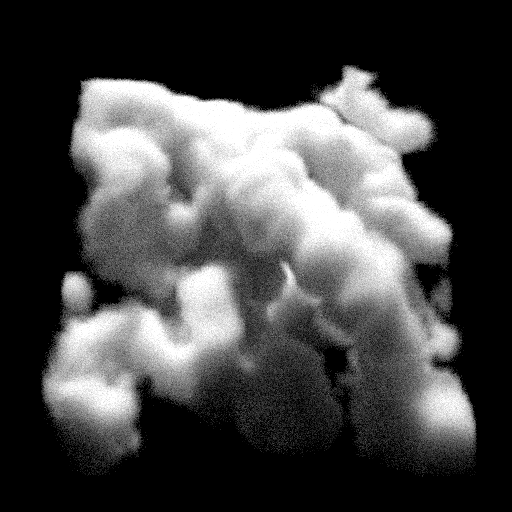
\includegraphics[width=\columnwidth]{06_fld/results/nebulae_ms_groundtruth.png}
\caption{Path-traced}
\label{fig:fld_results_nebulae_1}
\end{subfigure}
\hspace{0.01\columnwidth}
\begin{subfigure}[t]{0.48\columnwidth}
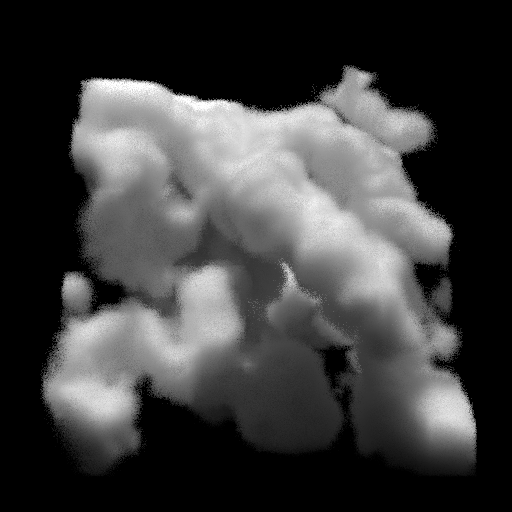
\includegraphics[width=\columnwidth]{06_fld/results/nebulae_ms_fld.png}
\caption{Flux-limited Diffusion}
\label{fig:fld_results_nebulae_2}
\end{subfigure}

\begin{subfigure}[t]{0.48\columnwidth}
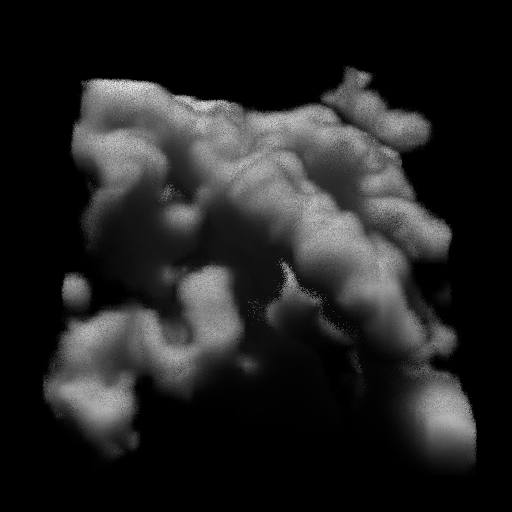
\includegraphics[width=\columnwidth]{06_fld/results/nebulae_ms_cda.png}
\caption{Diffusion Approximation}
\label{fig:fld_results_nebulae_3}
\end{subfigure}%
\hspace{0.01\columnwidth}
\begin{subfigure}[t]{0.48\columnwidth}
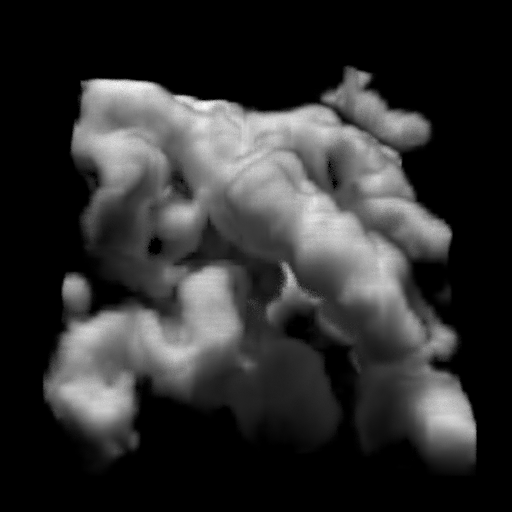
\includegraphics[width=\columnwidth]{06_fld/results/nebulae_ms_p5.png}
\caption{$P_5$}
\label{fig:fld_results_nebulae_4}
\end{subfigure}

%\vspace{-0.2in}
\caption{Flux-limited diffusion results for the procedural cloud dataset compared against previous methods. FLD produces results which are similarily close to the pathtraced solution than $P_5$ at a fraction of its computational cost.}
\label{fig:fld_results_nebulae}
\end{figure}

In terms of performance chacteristics it is to be expected that flux-limited diffusion requires more computational effort than the diffusion approximation, due to the non-linear nature of flux-limited diffusion coefficient, which must be updated for every voxel in each Gauss-Seidel iteration. This impact appears moderate when compared to the visual improvement it brings. When compared to $P_N$ it can be concluded that flux-limited diffusion offers a much better result at a significantly lower computational cost.

%\TD{complete table maybe table showing the performance characteristic for all three datasets}
%\TD{mention how the performance of FLD allows aplication of transfer function and solve for different color channels}
%\TD{mention publication}
%\TD{mention application in elementacular}